\documentclass[]{article}
\usepackage[dutch]{babel}
\usepackage{graphicx}
\usepackage{amsmath}
\usepackage[]{siunitx}
\usepackage{hyperref}
%opening
\title{Lab: Embedded system design 1}
\author{Thomas Feys \and Jona Cappelle}

\begin{document}

\maketitle

\newpage

\tableofcontents

\newpage

\section{Inleiding}
Ons doel is om de wachtrij in de rabotaria te monitoren. Dit zullen we doen aan de hand van een IR grid sensor (AMG8833). Aan de hand van de uitgelezen waarden zullen we in het tweede semester bepalen hoeveel mensen er in de wachtrij staan. Deze informatie zullen we vervolgens via een app of website verspreiden.


\section{Sensor}
De sensor die we gebruiken om de wachtrij te monitoren is de AMG8833. Deze IR grid sensor heeft 8x8 pixels die de temperatuur weergeven. Volgens de datasheet kan a.d.h.v. de temperatuur een mens waargenomen worden vanop een afstand van 5 meter. De sensor kan gebruikt worden in 3 verschillende modes: normal, sleep en stand-by. In de normale mode heeft de sensor een verbruik van 4.5 mA. De stand-by mode heeft twee opties; de waardes kunnen geüpdatet worden om de 60 seconden of om de 10 seconden. In deze mode is er een verbruik van 0.8 mA. Als laatste is er de sleep mode deze verbruikt 0.2 mA. Een overzicht van alle modes en de commando's die verstuurd moeten worden om in deze modes te raken wordt weergegeven in figuur \ref{fig:operatingmodes}. Tijdens het testen van de sensor hebben we periodiek geswitched tussen de verschillende power modes. Het resultaat van deze test is te zien in figuur \ref{fig:powertest}. De sensor heeft ook een interrupt pin. Deze pin geneert een interrupt als een van de pixels over of onder een bepaalde waarde gaat. Deze waarde is instelbaar.	
\begin{figure}[!ht]
	\centering
	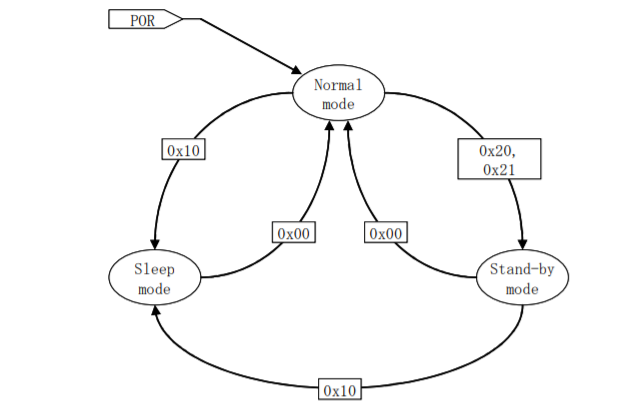
\includegraphics[width=\columnwidth]{operatingmodes.png}
	\caption{Overzicht operating modes}
	\label{fig:operatingmodes}
\end{figure}

%todo figuur aanpassen naar screenshot powermodes in de power monitor 
%todo test doen in verschillende modes met processor in sleep

\begin{figure}[!ht]
	\centering
	\includegraphics[width=\columnwidth]{power_modes_cycle_AMG8833_em2.png}
	\caption{Test van de verschillende powermodes}
	\label{fig:powertest}
\end{figure}

\section{Systeem}
\subsection{Overzicht}
De AMG8833 communiceert met de EFM32 via I2C. Naast de I2C communicatie is er ook een interrupt pin voorzien op de sensor. Deze pin genereert een interrupt als er een van de pixels een bepaalde, instelbare waarde overschrijdt. Een volledig overzicht van het systeem is te zien in figuur \ref{fig:systeem}.

\begin{figure}[!ht]
	\centering
	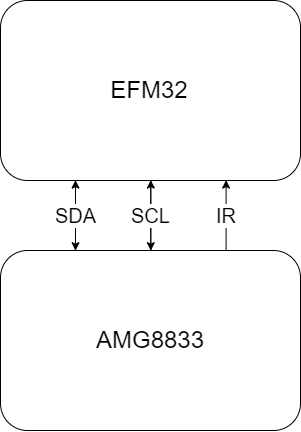
\includegraphics[scale=0.5]{sys.png}
	\caption{Overzicht van het systeem}
	\label{fig:systeem}
\end{figure}
\subsection{I2C}
De communicatie met de sensor gebeurt via I2C. Het adres van de sensor is een 7 bit adres namelijk: 1101001. Aangezien we met een 7 bit adres zitten moet deze 1 bit geshift worden naar links. Dit adres moet telkens naar de sensor verstuurd worden vooraleer er iets gelezen of geschreven kan worden. De code die gebruikt wordt om de sensor uit te lezen, in andere powermodus te zetten en te interrupten wordt in de volgende sectie besproken. 


\section{Code}
\subsection{Functionaliteiten}
Om gemakkelijk met de sensor te werken werd er een library geschreven voor de AMG8833. Er werden verschillende methodes geschreven om vlot te kunnen omgaan met de sensor. Er werd een functie geschreven om alle pixels uit te lezen. Naast de pixels is er ook een thermistor aanwezig in de sensor, ook hiervoor werd een functie geschreven. Er werden ook verschillende functies geschreven om makkelijk tussen de verschillende powermodes te kunnen wisselen. Een volledig overzicht van deze library en de rest van de code is terug te vinden op github: \url{https://github.com/jonacappelle/Embedded_Project}.


\subsection{Flow van de code}
\label{flowcode}
Om het verbruik te minimaliseren wordt er maar om de 5 minuten gecontroleerd of er mensen aanwezig zijn. Indien er mensen aanwezig zijn wordt de sensor in stand-by gezet en zal hij uitgelezen worden telkens als de sensor een interrupt genereert. De sensor genereert een interrupt als er minimum 1 pixel boven een bepaalde threshold ligt. Dit zal maar om de 60 seconden gebeuren aangezien de sensor zijn waarden maar update om de 60 seconden in stand-by mode. Indien er geen mensen aanwezig zijn, dan worden de sensor en de processor in sleep gezet. Deze zullen uit sleep gehaald worden als de timer weer afgaat. Een volledig overzicht van de code is terug te vinden in figuur \ref{fig:flowchart}.

\begin{figure}[!ht]
	\centering
	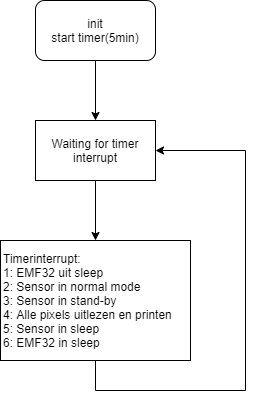
\includegraphics[scale=0.5]{flowchart.png}
	\caption{flowchart van de code}
	\label{fig:flowchart}
\end{figure}


\section{Power consumptie}
\subsection{Sensor}
De sensor heeft 3 verschillende powermodes, deze zijn te zien in figuur \ref{fig:sensor_power}. Deze hebben we ook zelf opgemeten zoals te zien is in figuur \ref{fig:powertest}. De gemeten waarden liggen in dezelfde grote orde als deze die opgegeven zijn in de datasheet, maar wijken toch een klein beetje af. In normal mode gebruikt onze sensor ... mA, in stand-by ... mA en in sleep ... mA.

\begin{figure}[!ht]
	\centering
	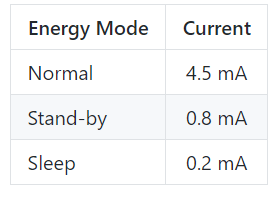
\includegraphics{sensor_power.png}
	\caption{powermodes van de sensor}
	\label{fig:sensor_power}
\end{figure}

\subsection{Principe}
\paragraph{Sensor: }
Door de methode toe te passen die besproken werd in section \ref{flowcode} wordt de power consumptie sterk verminderd. Wanneer er geen mensen aanwezig zijn, wordt de sensor in sleep gezet waardoor het verbruik 0.2 mAh is in plaats van 0.8 mAh in stand-by. Verder is het verbruik afhankelijk van hoe frequent er mensen in de wachtrij staan. In de berekeningen gaan we er van uit dat er enkel mensen aan het wachten zijn tussen 11u en 14u. In dit geval zal de sensor 3u per dag constant in stand-by staan aangezien er 3u lang mensen aanwezig zijn. Verder zal de sensor nog 21u in sleep staan. Dit levert een verbruik van: 


\begin{equation}
	\frac{3 \text{ h}\cdot 0.8 \text{ mAh} + 21 \text{ h}\cdot 0.2 \text{ mAh}}{24 \text{ h}} = 0.275 \text{ mAh}
\end{equation}

Indien deze methode niet toegepast wordt en we de sensor constant in stand-by laten staan is er een verbruik van 0.8 mAh. We bekomen dus een besparing van 65.625 \%. 
\paragraph{Processor: }

\subsection{Metingen}
\paragraph{Geen aanwezigheid: }
meting doen met geen aanwezigheid: sensor constant aan en uit

\paragraph{Aanwezigheid: }
meting doen met constant x waarden $>$ threshold


\section{Besluit }



\end{document}
